% Judul dokumen
\title{Buku Tugas Akhir ITS}
\author{Qalbi, Habibul Rahman}

% Pengaturan ukuran teks dan bentuk halaman dua sisi
\documentclass[10pt,twoside]{report}

% Pengaturan ukuran halaman dan margin
\usepackage[a5paper,top=25mm,left=25mm,right=20mm,bottom=25mm]{geometry}

% Pengaturan ukuran spasi
\usepackage[singlespacing]{setspace}

% Pengaturan format bahasa
\usepackage[indonesian]{babel}

% Pengaturan detail pada file PDF
\usepackage[pdfauthor={\@author},bookmarksnumbered,pdfborder={0 0 0}]{hyperref}

% Pengaturan jenis karakter
\usepackage[utf8]{inputenc}

% Pengaturan pewarnaan
\usepackage[table,xcdraw]{xcolor}

% Pengaturan kutipan artikel
\usepackage[numbers]{natbib}

% Package lainnya
\usepackage{changepage}
\usepackage{enumitem}
\usepackage{eso-pic}
\usepackage{etoolbox}
\usepackage{graphicx}
\usepackage{lipsum}
\usepackage{lmodern}
\usepackage{longtable}
\usepackage{tabularx}
\usepackage{wrapfig}

% Package keperluan pribadi
\usepackage{xurl}

% Definisi untuk "Hati ini sengaja dikosongkan"
\patchcmd{\cleardoublepage}{\hbox{}}{
  \thispagestyle{empty}
  \vspace*{\fill}
  \begin{center}\textit{[Halaman ini sengaja dikosongkan]}\end{center}
  \vfill}{}{}

% Pengaturan penomoran halaman
\usepackage{fancyhdr}
\fancyhf{}
\renewcommand{\headrulewidth}{0pt}
\pagestyle{fancy}
\fancyfoot[CE,CO]{\thepage}
\patchcmd{\chapter}{plain}{fancy}{}{}
\patchcmd{\chapter}{empty}{plain}{}{}

% Pengaturan format judul bab
\usepackage{titlesec}
\titleformat{\chapter}[display]{\bfseries\Large}{BAB \centering\Roman{chapter}}{0ex}{\vspace{0ex}\centering}
\titleformat{\section}{\bfseries\large}{\MakeUppercase{\thesection}}{1ex}{\vspace{1ex}}
\titleformat{\subsection}{\bfseries\large}{\MakeUppercase{\thesubsection}}{1ex}{}
\titleformat{\subsubsection}{\bfseries\large}{\MakeUppercase{\thesubsubsection}}{1ex}{}
\titlespacing{\chapter}{0ex}{0ex}{4ex}
\titlespacing{\section}{0ex}{1ex}{0ex}
\titlespacing{\subsection}{0ex}{0.5ex}{0ex}
\titlespacing{\subsubsection}{0ex}{0.5ex}{0ex}

% Pengaturan format potongan kode
\usepackage{listings}
\definecolor{comment}{RGB}{0,128,0}
\definecolor{string}{RGB}{255,0,0}
\definecolor{keyword}{RGB}{0,0,255}
\lstdefinestyle{codestyle}{
  commentstyle=\color{comment},
  stringstyle=\color{string},
  keywordstyle=\color{keyword},
  basicstyle=\footnotesize\ttfamily,
  numbers=left,
  numberstyle=\tiny,
  numbersep=5pt,
  frame=lines,
  breaklines=true,
  prebreak=\raisebox{0ex}[0ex][0ex]{\ensuremath{\hookleftarrow}},
  showstringspaces=false,
  upquote=true,
  tabsize=2,
}
\lstset{style=codestyle}

% Isi keseluruhan dokumen
\begin{document}

  % Sampul luar Bahasa Indonesia
  \newcommand\covercontents{sampul/konten-id.tex}
  \AddToShipoutPictureBG*{
  \AtPageLowerLeft{
    % Ubah nilai berikut jika posisi horizontal background tidak sesuai
    \hspace{-3.5mm}

    % Ubah nilai berikut jika posisi vertikal background tidak sesuai
    \raisebox{0mm}{
      
\includegraphics[width=\paperwidth,height=\paperheight]{sampul/gambar/sampul-luar.png}
    }
  }
}

% Menyembunyikan nomor halaman
\thispagestyle{empty}

% Pengaturan margin untuk menyesuaikan konten sampul
\newgeometry{
  top=95mm,
  left=25mm,
  right=20mm,
  bottom=25mm
}

\begin{flushleft}

  % Pemilihan font sans serif
  \sffamily

  % Pemilihan warna font putih
  \color{white}

  % Pemilihan font bold
  \fontseries{bx}
  \selectfont

  \input{\covercontents}

\end{flushleft}

\restoregeometry


  % Atur ulang penomoran halaman
  \setcounter{page}{1}

  % Sampul dalam Bahasa Indonesia
  \renewcommand\covercontents{sampul/konten-id.tex}
  \AddToShipoutPictureBG*{
  \AtPageLowerLeft{
    % Ubah nilai berikut jika posisi horizontal background tidak sesuai
    \hspace{-3.5mm}

    % Ubah nilai berikut jika posisi vertikal background tidak sesuai
    \raisebox{0mm}{
      
\includegraphics[width=\paperwidth,height=\paperheight]{sampul/gambar/sampul-dalam.png}
    }
  }
}

% Menyembunyikan nomor halaman
\thispagestyle{empty}

% Pengaturan margin untuk menyesuaikan konten sampul
\newgeometry{
  top=95mm,
  left=25mm,
  right=20mm,
  bottom=25mm
}

\begin{flushleft}

  % Pemilihan font sans serif
  \sffamily

  % Pemilihan font bold
  \fontseries{bx}
  \selectfont

  \input{\covercontents}

\end{flushleft}

\restoregeometry

  \clearpage
  \cleardoublepage

  % Sampul dalam Bahasa Inggris
  \renewcommand\covercontents{sampul/konten-en.tex}
  \AddToShipoutPictureBG*{
  \AtPageLowerLeft{
    % Ubah nilai berikut jika posisi horizontal background tidak sesuai
    \hspace{-3.5mm}

    % Ubah nilai berikut jika posisi vertikal background tidak sesuai
    \raisebox{0mm}{
      
\includegraphics[width=\paperwidth,height=\paperheight]{sampul/gambar/sampul-dalam.png}
    }
  }
}

% Menyembunyikan nomor halaman
\thispagestyle{empty}

% Pengaturan margin untuk menyesuaikan konten sampul
\newgeometry{
  top=95mm,
  left=25mm,
  right=20mm,
  bottom=25mm
}

\begin{flushleft}

  % Pemilihan font sans serif
  \sffamily

  % Pemilihan font bold
  \fontseries{bx}
  \selectfont

  \input{\covercontents}

\end{flushleft}

\restoregeometry

  \cleardoublepage

  % Pengaturan ukuran indentasi paragraf
  \setlength{\parindent}{2em}

  % Pengaturan ukuran spasi paragraf
  \setlength{\parskip}{1ex}

  % Pernyataan keaslian
  \begin{center}
  \large
  \textbf{PERNYATAAN KEASLIAN\\TUGAS AKHIR}
\end{center}

% Menyembunyikan nomor halaman
\thispagestyle{empty}

\vspace{2ex}

% Ubah paragraf-paragraf berikut sesuai dengan yang ingin diisi pada pernyataan keaslian

Dengan ini saya menyatakan bahwa isi sebagian maupun keseluruhan Tugas Akhir saya dengan judul “Klasifikasi Gerakan Mencuci Tangan Berbasis \emph{CNN}” adalah benar-benar hasil karya intelektual sendiri, diselesaikan tanpa menggunakan bahan-bahan yang tidak diizinkan dan bukan merupakan karya orang lain yang saya akui sebagai karya sendiri. 

Semua referensi yang dikutip maupun dirujuk telah ditulis secara lengkap pada daftar pustaka. 

Apabila ternyata pernyataan ini tidak benar, saya bersedia menerima sanksi sesuai dengan peraturan yang berlaku. 

\vspace{4ex}

\begin{flushright}
  \begin{tabular}[b]{c}
    % Ubah kalimat berikut sesuai dengan tempat, bulan, dan tahun penulisan
    Surabaya, Juni 2021\\
    \\
    \\
    \\
    \\
    % Ubah kalimat-kalimat berikut sesuai dengan nama dan NRP mahasiswa
	Habibul Rahman Qalbi \\
	NRP' 0721 17 4000 0022
  \end{tabular}
\end{flushright}

  \cleardoublepage

  % Lembar pengesahan
  \begin{center}
	\large
  \textbf{LEMBAR PENGESAHAN}
\end{center}

% Menyembunyikan nomor halaman
\thispagestyle{empty}

\begin{center}
  % Ubah kalimat berikut dengan judul tugas akhir
  \textbf{KLASIFIKASI GERAKAN MENCUCI TANGAN BERBASIS \emph{CNN}}
\end{center}

\begingroup
  % Pemilihan font ukuran small
  \small

  \begin{center}
    % Ubah kalimat berikut dengan pernyataan untuk lembar pengesahan
    Tugas Akhir ini disusun untuk memenuhi salah satu syarat memperoleh gelar Sarjana Teknik di Institut Teknologi Sepuluh Nopember Surabaya
  \end{center}

  \begin{center}
    % Ubah kalimat berikut dengan nama dan NRP mahasiswa
    Oleh: Habibul Rahman Qalbi (NRP. 0721 17 4000 0022)
  \end{center}

  \begin{center}
    % Ubah kalimat-kalimat berikut dengan tanggal ujian dan periode wisuda
    Tanggal Ujian : XX Juli 2021\\
    Periode Wisuda : September 2021
  \end{center}

  \begin{center}
    Disetujui Oleh:
  \end{center}

  \begingroup
    % Menghilangkan padding
    \setlength{\tabcolsep}{0pt}

    \noindent
    \begin{tabularx}{\textwidth}{X c}
      % Ubah kalimat-kalimat berikut dengan nama dan NIP dosen pembimbing pertama
      Dr. Eko Mulyanto Yuniarno, S.T., M.T.		& (Pembimbing I) \\
      NIP: 19680601 199512 1 000        		& ................................... \\
      &  \\
      &  \\
      % Ubah kalimat-kalimat berikut dengan nama dan NIP dosen pembimbing kedua
      Reza Fuad Rachmadi, S.T., M.T., Ph.D		& (Pembimbing II) \\
      NIP: 19850403 201212 1 000        		& ................................... \\
      &  \\
      &  \\
      % Ubah kalimat-kalimat berikut dengan nama dan NIP dosen penguji pertama
      Dr. Galileo Galilei, S.T., M.Sc.  		& (Penguji I) \\
      NIP: 15640215 164201 1 001       			& ................................... \\
      &  \\
      &  \\
      % Ubah kalimat-kalimat berikut dengan nama dan NIP dosen penguji kedua
      Friedrich Nietzsche, S.T., M.Sc.  		& (Penguji II) \\
      NIP: 18441015 190008 1 001       			& ................................... \\
      &  \\
      &  \\
      % Ubah kalimat-kalimat berikut dengan nama dan NIP dosen penguji ketiga
      Alan Turing, ST., MT.             		& (Penguji III) \\
      NIP: 19120623 195406 1 001        		& ................................... \\
    \end{tabularx}
  \endgroup

  \vspace{2ex}

  \begin{center}
    % Ubah kalimat berikut dengan jabatan kepala departemen
    Mengetahui, \\
    Kepala Departemen Teknik Dirgantara FTD - ITS \\

    \vspace{8ex}

    % Ubah kalimat-kalimat berikut dengan nama dan NIP kepala departemen
    \underline{Dr. Supeno Mardi Susiki Nugroho, S.T., M.Kom.} \\
    NIP. 19700313 199512 1 000
  \end{center}
\endgroup

  \cleardoublepage

  % Nomor halaman pembuka dimulai dari sini
  \pagenumbering{roman}

  % Abstrak Bahasa Indonesia
  \begin{center}
  \large\textbf{ABSTRAK}
\end{center}

\addcontentsline{toc}{chapter}{ABSTRAK}

\vspace{2ex}

\begingroup
  % Menghilangkan padding
  \setlength{\tabcolsep}{0pt}

  \noindent
  \begin{tabularx}{\textwidth}{l >{\centering}m{2em} X}
    % Ubah kalimat berikut dengan nama mahasiswa
    Nama Mahasiswa    &:& 	Habibul Rahman Qalbi\\

    % Ubah kalimat berikut dengan judul tugas akhir
    Judul Tugas Akhir &:&	Klasifikasi Gerakan Mencuci Tangan  \\
    				  & &	Berbasis \emph{CNN} \\

    % Ubah kalimat-kalimat berikut dengan nama-nama dosen pembimbing
    Pembimbing        &:& 1. Dr. Eko Mulyanto Yuniarno, S.T., M.T. \\
                      & & 2. Reza Fuad Rachmadi, S.T., M.T., Ph.D \\
  \end{tabularx}
\endgroup

% Ubah paragraf berikut dengan abstrak dari tugas akhir
Cuci tangan merupakan langkah awal dalam kesehatan, dengan mencuci tangan kita dapat mencegah penyebaran penyakit. Akan tetapi, masih banyak masyarakat yang tidak sadar akan tata cara mencuci tangan yang baik sehingga tidak bersih sepenuhnya. Pemanfaatan teknologi Deep Learning dapat menjadi solusi untuk mengetahui apakah masyarakat telah mencuci tangan dengan benar, menggunakan kamera sebagai input yang kemudian di proses menggunakan Algoritma \emph{Convolutional Neural network (CNN)} kita dapat mengkalisifikasikan gerakan - gerakan yang dilakukan pengguna saat mencuci tangan. Harapannya hasil penelitian ini dapat membantu dalam memantau dan memastikan apakah masyarakat mencuci tangan dengan benar.

% Ubah kata-kata berikut dengan kata kunci dari tugas akhir
Kata Kunci: Tangan, Kesehatan, Klasifikasi, \emph{CNN}.

  \cleardoublepage

  % Abstrak Bahasa Inggris
  \begin{center}
  \large\textbf{ABSTRACT}
\end{center}

\addcontentsline{toc}{chapter}{ABSTRACT}

\vspace{2ex}

\begingroup
  % Menghilangkan padding
  \setlength{\tabcolsep}{0pt}

  \noindent
  \begin{tabularx}{\textwidth}{l >{\centering}m{3em} X}
    % Ubah kalimat berikut dengan nama mahasiswa
    \emph{Name}     &:&	Habibul Rahman Qalbi\\

    % Ubah kalimat berikut dengan judul tugas akhir dalam Bahasa Inggris
    \emph{Title}    &:& \emph{CNN} Based Hand Washing Motion Classification \\

    % Ubah kalimat-kalimat berikut dengan nama-nama dosen pembimbing
    \emph{Advisors} &:& 1. Dr. Eko Mulyanto Yuniarno, S.T., M.T. \\
    				& & 2. Reza Fuad Rachmadi, S.T., M.T., Ph.D \\
  \end{tabularx}
\endgroup

% Ubah paragraf berikut dengan abstrak dari tugas akhir dalam Bahasa Inggris
\emph{Abstract—Hand Washing is the first step when it comes to maintain health and hygine, by doing so we prevent the spread of deseases. Even though, there is still many people that didn’t wash their hand properly. By using Deep Learning algorithm, we could know if someone had wash their hand properly by capturing their movement with a camera and processing the data through a CNN Model. We hope that this technology could help to monitor and ensure that people had wash their hand properly, specially on public places where the potential spread of diseases is quite high.}

% Ubah kata-kata berikut dengan kata kunci dari tugas akhir dalam Bahasa Inggris
\emph{Keywords}: \emph{Hand}, \emph{Health}, \emph{Classification}, \emph{CNN}.

  \cleardoublepage

  % Kata pengantar
  \begin{center}
  \Large
  \textbf{KATA PENGANTAR}
\end{center}

\addcontentsline{toc}{chapter}{KATA PENGANTAR}

\vspace{2ex}

% Ubah paragraf-paragraf berikut dengan isi dari kata pengantar
Puji dan syukur kehadirat Allah Swt. atas segala limpahan berkah, rahmat, serta hidayah-Nya, penulis dapat menyelesaikan penelitian ini dengan judul "Klasifikasi Gerakan Mencuci Tangan Berbasis \emph{Convolutional Neural Network (CNN)}

Penelitian ini disusun dalam rangka pemenuhan bidang riset di Departemen Teknik Komputer, serta digunakan sebagai persyaratan menyelesaikan pendidikan S1. Penelitian ini dapat terselesaikan tidak lepas dari bantuan berbagai pihak. Oleh karena itu, penulis mengucapkan terima kasih kepada:

\begin{enumerate}[nolistsep]

  \item Bunda dan Ayah tercinta yang didalam setiap nafasnya selalu memberi dukungan, semangat dan do'a demi pendidikan, kehidupan dan masa depan anak - anaknya.

  \item Keluarga dan Saudara yang selalu memberi semangat dalam menjalani masa perkuliahan dan tugas akhir.
  
  \item Bapak Dr. Supeno Mardi Susiki Nugroho, ST., MT. selaku Kepala Departemen Teknik komputer sekaligus dosen pengampu mata kuliah Tugas Akhir yang telah memberi arahan pada pengerjaan tugas akhir ini.

  \item Bapak Dr. Eko Mulyanto Yuniarno, S.T., M.T selaku dosen pembimbing 1 (Satu) dan Bapak Reza Fuad Rachmadi, S.T., M.T., Ph.D selaku dosen pembimbing 2 (Dua) yang memberikan arahan dan dukungan dalam penelitian Tugas Akhir ini
  
  \item Bapak-ibu dosen pengajar Departemen Teknik Komputer, atas pengajaran, bimbingan, serta perhatian yang diberikan kepada penulis selama ini.
  
  \item Seluruh keluarga besar Tiyang Alit, serta teman - teman Teknik Komputer dan e57
  
  \item Sita Nuraini, yang memberikan dorongan dan motivasi selama pengerjaan tugas akhir ini.
  
  \item Teman-teman kos yang menjadi tempat berbagi cerita mengenai hiruk pikuk dunia perkuliahan.

\end{enumerate}

\newpage
Kesempurnaan hanya milik Allah SWT, untuk itu penulis memohon segenap kritik dan saran yang membangun, semoga penelitian ini dapat memberikan manfaat bagi kita semua.

\begin{flushright}
  \begin{tabular}[b]{c}
    % Ubah kalimat berikut dengan tempat, bulan, dan tahun penulisan
    Surabaya, Mei 2021\\
    \\
    \\
    \\
    \\
    % Ubah kalimat berikut dengan nama mahasiswa
    Habibul Rahman Qalbi
  \end{tabular}
\end{flushright}

  \cleardoublepage

  % Daftar isi
  \renewcommand*\contentsname{DAFTAR ISI}
  \addcontentsline{toc}{chapter}{\contentsname}
  \tableofcontents
  \cleardoublepage

  % Daftar gambar
  \renewcommand*\listfigurename{DAFTAR GAMBAR}
  \addcontentsline{toc}{chapter}{\listfigurename}
  \listoffigures
  \cleardoublepage

  % Daftar tabel
  \renewcommand*\listtablename{DAFTAR TABEL}
  \addcontentsline{toc}{chapter}{\listtablename}
  \listoftables
  \cleardoublepage

  % Nomor halaman isi dimulai dari sini
  \pagenumbering{arabic}

  % Bab 1 pendahuluan
  \chapter{PENDAHULUAN}
\label{chap:pendahuluan}

% Ubah bagian-bagian berikut dengan isi dari pendahuluan

Penelitian ini di latar belakangi oleh berbagai kondisi yang menjadi acuan. Selain itu juga terdapat beberapa permasalahan yang akan dijawab sebagai luaran dari penelitian.

\section{Latar Belakang}
\label{sec:latarbelakang}

Menjaga kebersihan merupakan salah satu kunci untuk menjaga kesehatan tubuh, tubuh yang bersih dapat menghindarkan kita dari berbagai penyakit terutama yang berasal dari lingkungan disekitar kita. Kita sering kali menyentuh benda - benda di sekitar seperti gadget, komputer, gagang pintu, meja, lemari, dan lain sebagainya. Akan tetapi, banyak yang tidak sadar bahwa benda benda tersebut seringkali menjadi sarang bagi bakteri \& virus yang dapat menyebabkan penyakit. 

Ketika menyentuh benda benda tersebut, kuman – kuman yang ada akan berpindah dan menyebar di tangan kita, kemudian ketika kita menyentuh orang lain, maka kuman penyebab penyakit itu akan berpindah dan menyebar ke tubuh orang tersebut. Pada akhirnya Ketika kita menyentuh bagian – bagian di tubuh seperti mata, hidung dan mulut, maka kuman tersebut akan masuk ke tubuh kita dan menyebabkan penyakit. Oleh karena itu mencuci tangan merupakan hal yang paling utama dalam menjaga kesehatan tubuh dan mencegah penyebaran penyakit.

Pada saat penelitian ini berlangsung, 2020 - 2021, sedang marak terjadinya pandemi virus SARS-CoV-2 (Severe Acute Respiratory Syndrome – Corona Virus – 2) atau yang biasa disebut COVID-19 (Corona Virus Desease – 2019)\cite{cit:copid}. Bahkan pada hari ini, 8 Juni 2021, tercatat 174,429,426 kasus COVID-19 di dunia dan 3,753,525 diantaranya meninggal dunia \cite{cit:covidcase}

\newpage
\begin{figure}[ht]
	\centering
	
	% Ubah dengan nama file gambar dan ukuran yang akan digunakan
	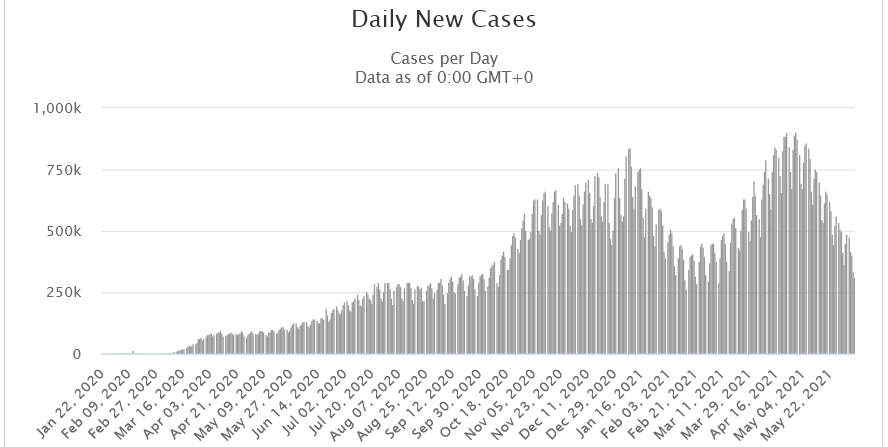
\includegraphics[width=0.9\columnwidth]{gambar/worldometer.PNG}
	
	% Ubah dengan keterangan gambar yang diinginkan
	\caption{Grafik Perkembangan Kasus \emph{COVID-19} \citep{cit:covidcase}.}
	\label{fig:covidstat}
\end{figure}

Virus ini menyerang sistem pernafasan yang menyebabkan pengidapnya kesulitan bernafas, kekurangan oksigen, hingga kematian. Virus ini sangat mudah untuk menyebar terutama melalui \emph{droplets} (percikan air) yang terjadi ketika bersin, batuk, dan bicara sekalipun. Droplets ini akan menempel ke benda - benda dan tubuh kita. Hanya dengan menyentuh benda atau bagian tubuh yang terkontaminasi kemudian tanpa sadar menyentuh mata, hidung ataupun mulut, maka virus tersebut akan masuk ke tubuh dan merusak sel paru-paru yang akhirnya menyebabkan gangguan pernafasan bahkan kematian.

Walaupun kebiasaan cuci tangan meningkat selama pandemi COVID-19 \cite{cit:cucisabun} banyak orang yang masih asal – asalan ketika mencuci tangan lantaran terburu-buru maupun hal lainnya. Menurut hallosehat.com \cite{cit:salahcuci} , masih banyak kesalahan dalam mencuci tangan yang sering dilakuk-an oleh masyarakat, diantaranya waktu mencuci tangan yang terlalu cepat dan kebiasaan masyarakat yang hanya menggosok talapak tangan saja ketika sedang mencuci tangan. Akan tetapi tidak memung-kinkan untuk dilakukannya pemantauan 7x24 jam oleh manusia terhadap pengunjung di tempat umum seperti mall dan tempat wisata lainnya demi memastikan pengunjung telah mencuci tangan dengan be-nar, terutama di masa pandemi COVID-19 ini yang mana masyarakat dihimbau untuk menjaga jarak untuk mencegah penularan.

\section{Permasalahan}
\label{sec:permasalahan}

Dari permasalahan tersebut maka permasalahan yang di ambil dalam penelitian tugas akhir ini adalah menemukan cara mendeteksi apakah seseorang sudah mencuci tangan dengan baik. Untuk itu diperlukan sebuah sistem klasifikasi gerakan mencuci tangan yang kemudian dapat dikembangkan lagi untuk menilai apakah orang tersebut telah mencuci tangannya dengan baik dan benar tanpa perlu dilakukannya pemantauan langsung oleh manusia

\section{Tujuan}
\label{sec:Tujuan}

Tujuan dari tugas akhir ini adalah membuat sebuah sistem yang dapat mengklasifikasikan gerakan mencuci tangan

\section{Batasan Masalah}
\label{sec:batasanmasalah}

Untuk memfokuskan permasalahan yang diangkat maka dilakukan pembatasan masalah. Batasan-batasan masalah tersebut di antaranya adalah:

\begin{enumerate}[nolistsep]
	
  \item Sistem Hanya berfokus pada Klasifikasi Gerakan Mencuci Tangan
  
  \item Metode Klasifikasi yang digunakan adalah metode \emph{Image Classification} berbasis CNN dengan mengaplikasikan Moving Average pada hasil prediksinya 
  
  \item \emph{Base Model} dalam Klasifikasi ini menggunakan \emph{EfficientNet}\cite{cit:effnet} dengan \emph{Weight Checkpoint} \emph{NoisyStudent}\cite{cit:noisy}
  
  \item Dataset yang digunakan berasal dari Kaggle Hand Wash Dataset Sample dan Dataset Pribadi

  \item Metode pengambilan data pribadi adalah menggunakan satu kamera dengan posisi dan sudut yang tetap
  
  \item Dikarenakan Kondisi Pandemi COVID-19 \cite{cit:copid}, Penelitian hanya akan dilakukan di sekitar tempat tinggal penulis dengan menerapkan \emph{Physical Distancing} demi mencegah terjadinya penyebaran penyakit
  
\end{enumerate}

\newpage
\section{Sistematika Penulisan}
\label{sec:sistematikapenulisan}

Laporan penelitian tugas akhir ini tersusun dalam sistematika dan terstruktur sehingga mudah dipahami dan dipelajari oleh pembaca maupun seseorang yang ingin melanjutkan penelitian ini. Alur sistematika penulisan laporan penelitian ini yaitu:

\begin{enumerate}[nolistsep]

  \item \textbf{BAB I Pendahuluan}

  Bab ini berisi uraian tentang latar belakang permasalahan, penegasan dan alasan pemilihan judul, sistematika laporan, tujuan, dan metodologi penelitian.
  
  \vspace{2ex}

  \item \textbf{BAB II Tinjauan Pustaka}

  Bab ini berisi tentang uraian secara sistematis teori-teori yang berhubungan dengan permasalahan yang dibahas pada penelitian ini. Teori-teori ini digunakan sebagai dasar dalam penelitian, yaitu informasi terkait Deep Learning, Convolutional Neural Network (CNN), EfficientNet dan teori-teori penunjang lainya.

  \vspace{2ex}

  \item \textbf{BAB III Desain dan Implementasi Sistem}

  Bab ini berisi tentang penjelasan-penjelasan terkait eksperimen yang akan dilakukan, langkah-langkah pengambilan data video dan proses klasifikasi gerakan mencuci tangan, serta analisis performa dari sistem. Guna mendukung itu digunakanlah blok diagram atau workflow agar sistem yang akan dibuat dapat terlihat dan mudah dibaca untuk implementasi pada pelaksanaan tugas akhir.

  \vspace{2ex}

  \item \textbf{BAB IV Pengujian dan Analisa}

  Bab ini menjelaskan tentang hasil serta analisis yang dida-patkan dari pengujian yang dilakukan mulai dari hasil pengujian \emph{model.evaluation}, \emph{Confusion Matrix}, Pengujian pada video cuci tangan serta rekomendasi penerapan sistem.

  \vspace{2ex}

  \item \textbf{BAB V Penutup}

  Bab ini merupakan penutup yang berisi kesimpulan yang di-ambil dari penelitian dan pengujian yang telah dilakukan. Sar-an dan kritik yang membangun untuk pengembangan lebih lanjut juga dituliskan pada bab ini.

\end{enumerate}

  \cleardoublepage

  % Bab 2 tinjauan pustaka
  \chapter{TINJAUAN PUSTAKA}
\label{chap:tinjauanpustaka}

% Ubah bagian-bagian berikut dengan isi dari tinjauan pustaka

Demi mendukung penelitian ini, dibutuhkan beberapa teori penunjang sebagai bahan acuan dan referensi. Dengan demikian penelitian ini menjadi lebih terarah.

\section{Convolutional Neural Network (CNN)}
\label{sec:cnn}

\emph{Convolutional Neural Network (CNN)} adalah salah satu jenis neural network yang biasa digunakan pada data image \cite{cit:cnn}. CNN bisa digunakan untuk mendeteksi dan mengenali object pada sebuah image. CNN adalah sebuah teknik yang terinspirasi dari cara mamalia — manusia, menghasilkan persepsi visual seperti yang terlihat pada gambar \ref{fig:kudakudaan}.

Secara garis besar Convolutional Neural Network (CNN) tidak jauh berbeda dengan neural network biasanya. CNN terdiri dari neuron yang memiliki weight, bias dan activation function. 

\begin{figure}[ht]
	\centering
	
	% Ubah dengan nama file gambar dan ukuran yang akan digunakan
	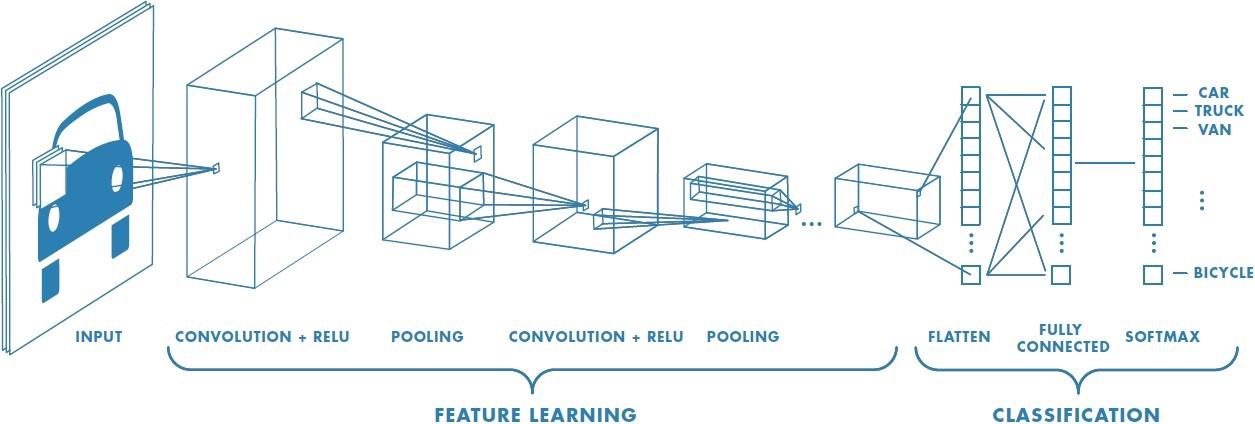
\includegraphics[width=1\columnwidth]{gambar/cnn.jpeg}
	
	% Ubah dengan keterangan gambar yang diinginkan
	\caption{Arsitektur CNN \citep{cit:cnn}}
	\label{fig:cnn}
\end{figure}

Yang membedakan CNN dari Neural network lainnya terletak pada Arsitektur dari CNN itu sendiri. Arsitektur dari CNN dibagi menjadi 2 bagian besar, \textit{\textbf{Feature Learning Layer}} dan \textit{\textbf{Classification Layer}}.

\subsection{Feature Learning}
\label{subsec:featurelearning}

Pada bagian ini CNN akan melakukan “encoding” dari sebuah image menjadi features yang berupa angka-angka yang merepresentasikan image tersebut, maka dari itu bagian ini sering juga disebut \textit{Feature Extraction Layer}. Feature Learning terdiri dari dua bagian. Convolutional Layer, Activation dan Pooling Layer.

\begin{enumerate}
	\item \textit{Convolutional Layer (Conv. Layer)}
	\begin{figure}[ht]
		\centering
		
		% Ubah dengan nama file gambar dan ukuran yang akan digunakan
		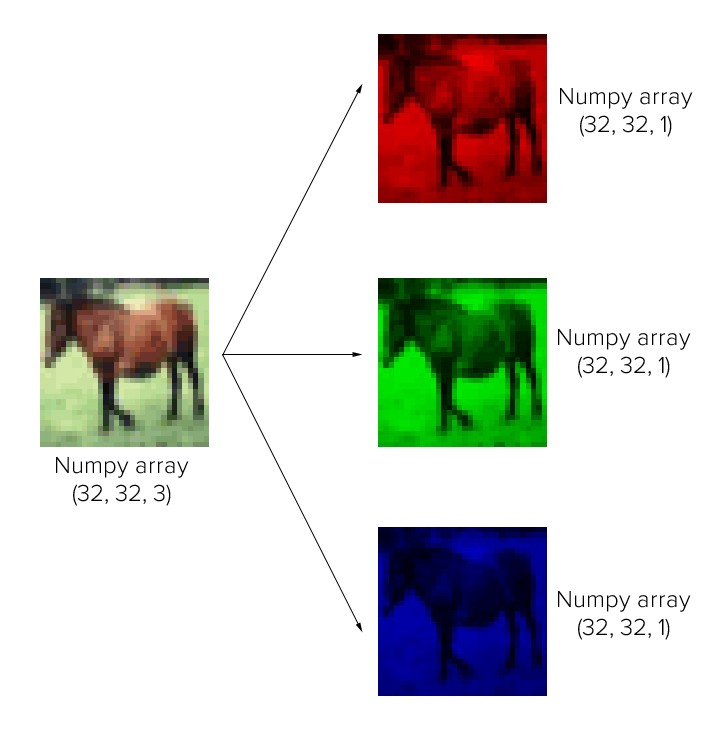
\includegraphics[width=0.7\columnwidth]{gambar/rgbhorse.jpeg}
		
		% Ubah dengan keterangan gambar yang diinginkan
		\caption{Contoh Citra RGB\citep{cit:cnn}}
		\label{fig:kudargb}
	\end{figure}
	
	Gambar \ref{fig:kudargb} adalah Citra RGB (Red, Green, Blue) berukuran 32x32 pixels yang sebenarnya adalah multidimensional array dengan ukuran 32x32x3 (3 adalah jumlah channel).
	
	Convolutional layer terdiri dari neuron yang tersusun sedemikian rupa sehingga membentuk sebuah filter dengan panjang dan tinggi (pixels). Sebagai contoh, layer pertama pada feature extraction layer biasanya adalah convolutional layer dengan ukuran 5x5x3. Panjang 5 pixels, tinggi 5 pixels dan tebal/jumlah 3 buah sesuai dengan channel dari image tersebut.
	
	Ketiga filter ini akan digeser keseluruh bagian dari gambar. Setiap pergeseran akan dilakukan operasi “dot” antara input dan nilai dari filter tersebut sehingga menghasilkan sebuah output atau biasa disebut sebagai activation map atau feature map.
	
	\begin{figure}[h]
		\centering
		
		% Ubah dengan nama file gambar dan ukuran yang akan digunakan
		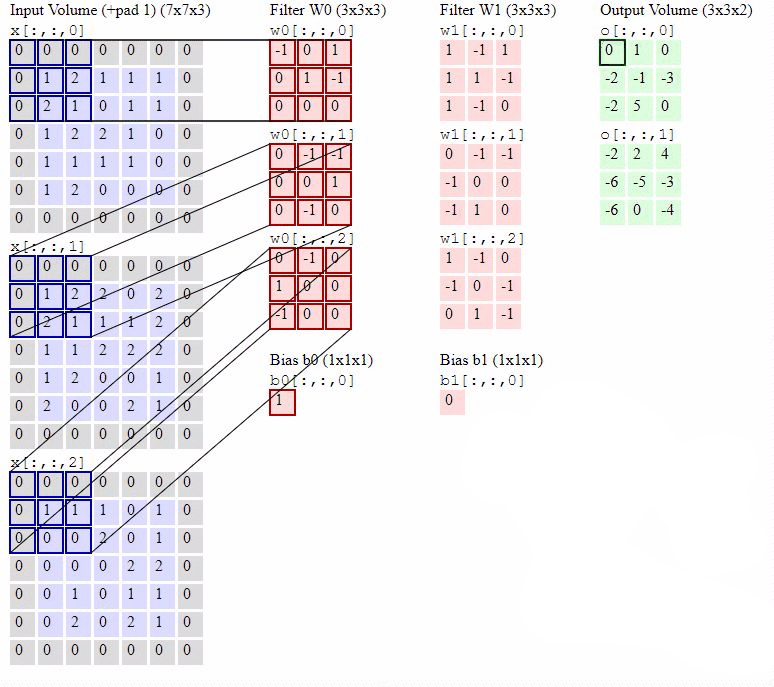
\includegraphics[width=0.9\columnwidth]{gambar/convpool.png}
		
		% Ubah dengan keterangan gambar yang diinginkan
		\caption{Convolutional Layer\citep{cit:cnn}}
		\label{fig:convolutionallayer}
	\end{figure}

	Terdapat berberapa bagian didalam Convolutional Layer, diantaranya sebagai berikut:
	
	\begin{itemize}
		\item \textit{Stride}
		
		Stride adalah parameter yang menentukan berapa jumlah pergeseran filter. Jika nilai stride adalah 1, maka conv. filter akan bergeser sebanyak 1 pixels secara horizontal lalu vertical. Pada ilustrasi diatas, stride yang digunakan adalah 2.
		
		Semakin kecil stride maka akan semakin detail informasi yang kita dapatkan dari sebuah input, namun membutuhkan komputasi yang lebih jika dibandingkan dengan stride yang besar.
		
		Namun perlu diperhatikan bahwa dengan menggunakan stride yang kecil kita tidak selalu akan mendapatkan performa yang bagus.
		
		\item \textit{Padding}
		
		Padding atau Zero Padding adalah parameter yang menentukan jumlah pixels (berisi nilai 0) yang akan ditambahkan di setiap sisi dari input. Hal ini digunakan dengan tujuan untuk memanipulasi dimensi output dari conv. layer (Feature Map).
		
		Tujuan dari penggunaan padding adalah :
		\begin{enumerate}
			\item Dimensi output dari conv. layer selalu lebih kecil dari inputnya (kecuali penggunaan 1x1 filter dengan stride 1). Output ini akan digunakan kembali sebagai input dari conv. layer selanjutnya, sehingga makin banyak informasi yang terbuang.
			
			Dengan menggunakan padding, kita dapat mengatur dimensi output agar tetap sama seperti dimensi input atau setidaknya tidak berkurang secara drastis. Sehingga kita bisa menggunakan conv. layer yang lebih dalam/deep sehingga lebih banyak features yang berhasil di-extract.
			
			\item Meningkatkan performa dari model karena conv. filter akan fokus pada informasi yang sebenarnya yaitu yang berada diantara zero padding tersebut.
		\end{enumerate}
		
		Pada ilustrasi \ref{fig:convolutionallayer}, dimensi dari input sebenarnya adalah 5x5, jika dilakukan convolution dengan filter 3x3 dan stride sebesar 2, maka akan didapatkan feature map dengan ukuran 2x2. Namun jika kita tambahkan zero padding sebanyak 1, maka feature map yang dihasilkan berukuran 3x3 (lebih banyak informasi yang dihasilkan).
		
		\newpage
		Untuk menghitung dimensi dari feature map kita bisa gunakan rumus \ref{eq:featuremap} sebagai berikut.
		
		\begin{equation}
			\label{eq:featuremap}
			output = \frac{W-N+2P}{S} + 1
		\end{equation}
		\subitem \textit{W} = Panjang/Tinggi Input
		\subitem \textit{N} = Panjang/Tinggi Filter
		\subitem \textit{P} = Zero Padding
		\subitem \textit{S} = Stride
		
	\end{itemize}

	\item \textit{Activation Layer}
	
	Setelah melalui convolution layer, nilai hasil konvolusi dikenakan fungsi aktivasi. Terdapat beberapa fungsi aktivasi yang sering digunakan pada convolutional network, di antaranya tanh() atau ReLU. Aktivasi ReLU menjadi pilihan bagi beberapa peneliti karena sifatnya yang lebih berfungsi dengan baik pada klasifikasi citra.
	
	Fungsi aktifasi ReLU adalah Fungsi maks (x,0). Jika input dari fungsi aktivasi adalah negatif maka nilai output dari neuron bisa dinyatakan sebagai 0, tapi jika nilai input dari fungsi aktivasi adalah positif maka output dari neuron adalah nilai input aktivasi itu sendiri.
	
	\item \textit{Pooling Layer}
	
	Pooling layer biasanya berada setelah conv. layer. Pada prinsipnya pooling layer terdiri dari sebuah filter dengan ukuran dan stride tertentu yang akan bergeser pada seluruh area feature map.
	
	Pooling yang biasa digunakan adalah Max Pooling dan Average Pooling. Sebagai contoh jika kita menggunakan Max Pooling 2x2 dengan stride 2, maka pada setiap pergeseran filter, nilai maximum pada area 2x2 pixel tersebut yang akan dipilih, sedangkan Average Pooling akan memilih nilai rata-ratanya.
	
	\begin{figure}[h]
		\centering
		
		% Ubah dengan nama file gambar dan ukuran yang akan digunakan
		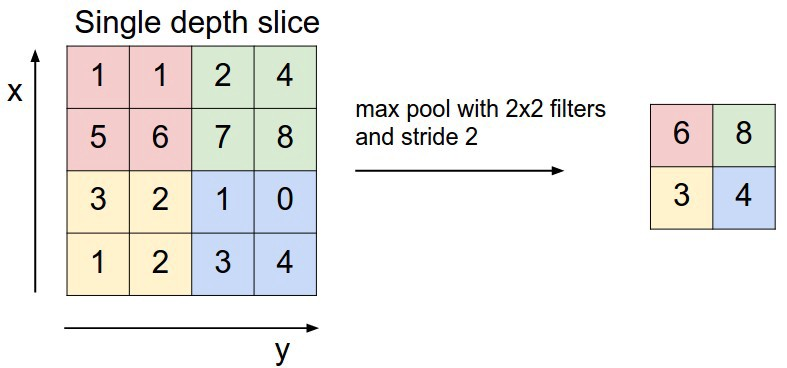
\includegraphics[width=0.7\columnwidth]{gambar/poolinglayer.jpeg}
		
		% Ubah dengan keterangan gambar yang diinginkan
		\caption{Pooling Layer\citep{cit:cnn}}
		\label{fig:poolinglayer}
	\end{figure}	
	
	Tujuan dari penggunaan pooling layer adalah mengurangi dimensi dari feature map (downsampling), sehingga mempercepat komputasi karena parameter yang harus diupdate semakin sedikit dan mengatasi overfitting.
\end{enumerate}

\vspace{2ex}
\subsection{Classification}
\label{subsec:classification}

\textit{Classification Layer} adalah bagian dari neural network yang memproses hasil dari Feature-Extraction (Feature Learning) Layer dan memberikan output berupa hasil prediksi atau klasifikasi. \textit{Classification layer} Memiliki 3 bagian Utama yaitu Flatten, Fully-Connected dan Activation.

\begin{enumerate}
	\item \textit{Flatten}
	
	Feature map yang dihasilkan dari feature extraction layer masih berbentuk multidimensional array, sehingga kita harus melakukan “flatten” atau reshape feature map menjadi sebuah vector untuk kemudian dapat diproses pada fully-connected layer.
	
	\item \textit{Fully-connected}
	
	Lapisan Fully-connected adalah lapisan dimana semua neuron aktivitas dari lapisan sebelumnya terhubung semua dengan neuron di lapisan selanjutnya seperti hal nya jaringan syaraf tiruan bisa. Setiap aktivitas dari lapisan sebelumnya perlu diubah menjadi data satu dimensi sebelum dapat dihubungkan ke semua neuron di lapisan Fully-Connected.
	
	Lapisan Fully-Connected biasanya digunakan pada metode \textit{Multi Layer Perceptron} dan bertujuan untuk mengolah data sehingga bisa diklasifikasikan. Perbedaan anatar lapisan Fully-Connected dan lapisan konvolusi biasa adalah neuron di Convolution Layer terhubung hanya ke daerah tertentu pada input. Sementara lapisan Fully-Connected memiliki neuron yang secara keseluruhan terhubung. Namun, kedua lapisan tersebut masih menggunakan operasi "dot", sehinga fungsinya tidak begitu berbeda.
	
	\item \textit{Activation}
	
	\textit{Activation layer} pada \textit{Classification} sedikit berbeda dengan yang ada pada \textit{Feature Learning} (\textit{section} \ref{subsec:featurelearning}). Fungsi yang digunakan adalah fungsi Softmax. Fungsi Softmax mengambil output dari Fully-connected layer, menggabungkannya, dan memberikan output berupa hasil klasifikasi secara keseluruhan dalam bentuk probabilitas dalam rentang nilai 0 s.d 1.
	
\end{enumerate}

\vspace{2ex}
\section{EfficientNet}
\label{sec:effnet}

\textit{EfficientNet} adalah arsitektur CNN yang dikembangkan dengan menggunakan \textit{Compound Scaling}. Tidak seperti Model \textit{Transfer Learning} pada umumnya, EfficientNet dikembangkan dengan melakukan \textit{Scaling} pada Kedalaman, Lebar, dan Resolusi model. \cite{cit:effnet}

\vspace{2ex}
\subsection{Arsitektur EfficientNet}
\label{subsec:arsitekturefn}
Varian dasar dari Model EfficientNet yaitu EfficientNet-B0 dikembangkan dari model sebelumnya sebagai model dasar. Pemilihan model dasar ini dilakukan secara otomatis menggunakan AutoML MNAS. 

\begin{figure}[h]
	\centering
	
	% Ubah dengan nama file gambar dan ukuran yang akan digunakan
	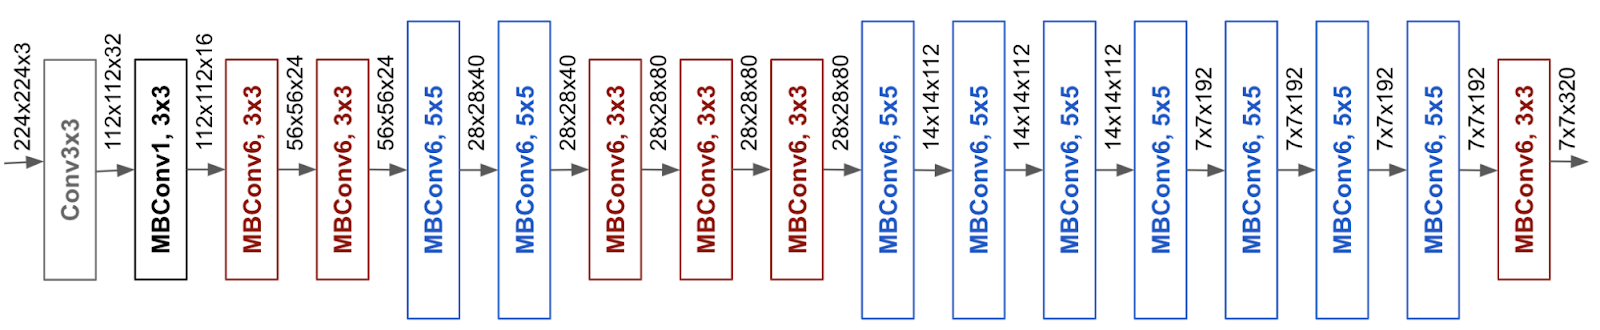
\includegraphics[width=1\columnwidth]{gambar/arsitekturefn.png}
	
	% Ubah dengan keterangan gambar yang diinginkan
	\caption{Arsitektur EfficientNet \citep{cit:effnet}}
	\label{fig:arsitektur-efn}
\end{figure}


AutoML MNAS berkerja dengan mencoba untuk mencapai akurasi tertinggi dari suatu permasalah klasifikasi (yang dalam hal ini \textit{imagenet}) dengan mencari dan menggabungkan arsitektur dari model - model yang telah ada sebelumnya secara otomatis berdasarkan skor yang mereka hasilkan melalui perbandingan Tingkat Akurasi dan Resource yang diperlukan. Dalam hal ini, model paling efisien dicapai dengan menggunakan MobileNetv2 dengan Menambahkan (squeeze-and-excitation block) ke dalamnya.

\vspace{2ex}
\subsection{Compound Scaling}
\label{subsec:compoundscaling}
\begin{figure}[h]
	\centering
	
	% Ubah dengan nama file gambar dan ukuran yang akan digunakan
	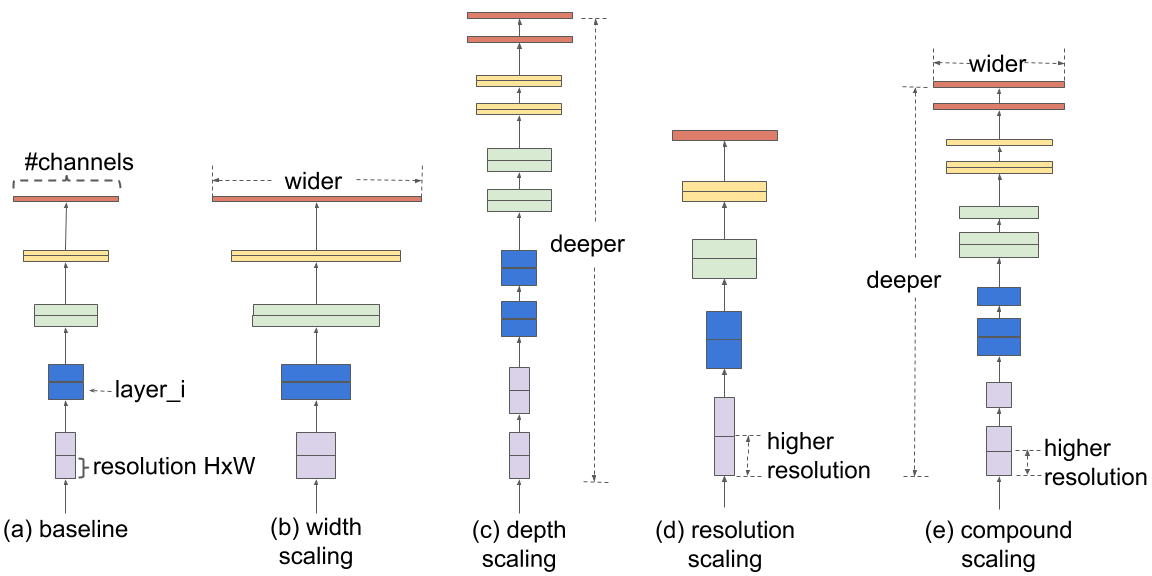
\includegraphics[width=0.9\columnwidth]{gambar/modelscaling.png}
	
	% Ubah dengan keterangan gambar yang diinginkan
	\caption{Comparison of CNN Model Scaling \citep{cit:effnet}}
	\label{fig:modelscaling}
\end{figure}

Setelah Didapat varian dasarnya (EfficientNet-B0), Compound Scaling kemudian diterapkan untuk menciptakan EfficientNet-B1 Hingga EfficientNet-B7. Dengan begitu model dengan efisien bisa didapatkan dengan menggunakan resource terbatas.

Hal ini terbukti dengan menggunakan Compound Scaling pada model sebelumnya seperti MobileNet (+1.4\% Akurasi \textit{imagenet}) dan ResNet (+0.7\% Akurasi) jika dibandingkan dengan metode scaling konvensional \cite{cit:effnet}

\vspace{2ex}
\subsection{Performa EfficientNet}
\label{subsec:efn-perf}

Pada klasifikasi dataset \textit{ImageNet} dibandingkan dengan model CNN yang telah ada sebelumnya, secara keseluruhan EfficientNet mencapai hasil akurasi dan efisiensi yang lebih baik. Bahkan, EfficientNet-B7 mencapai tingkat akurasi 84.4\% top-1 / 97.1\% top-5 pada dataset \textit{ImageNet}. ini membuat EfficientNet memiliki tingkat akurasi \textit{state-of-the-art} dari \textit{ImageNet} pada saat itu (2019)

\begin{figure}[h]
	\centering
	
	% Ubah dengan nama file gambar dan ukuran yang akan digunakan
	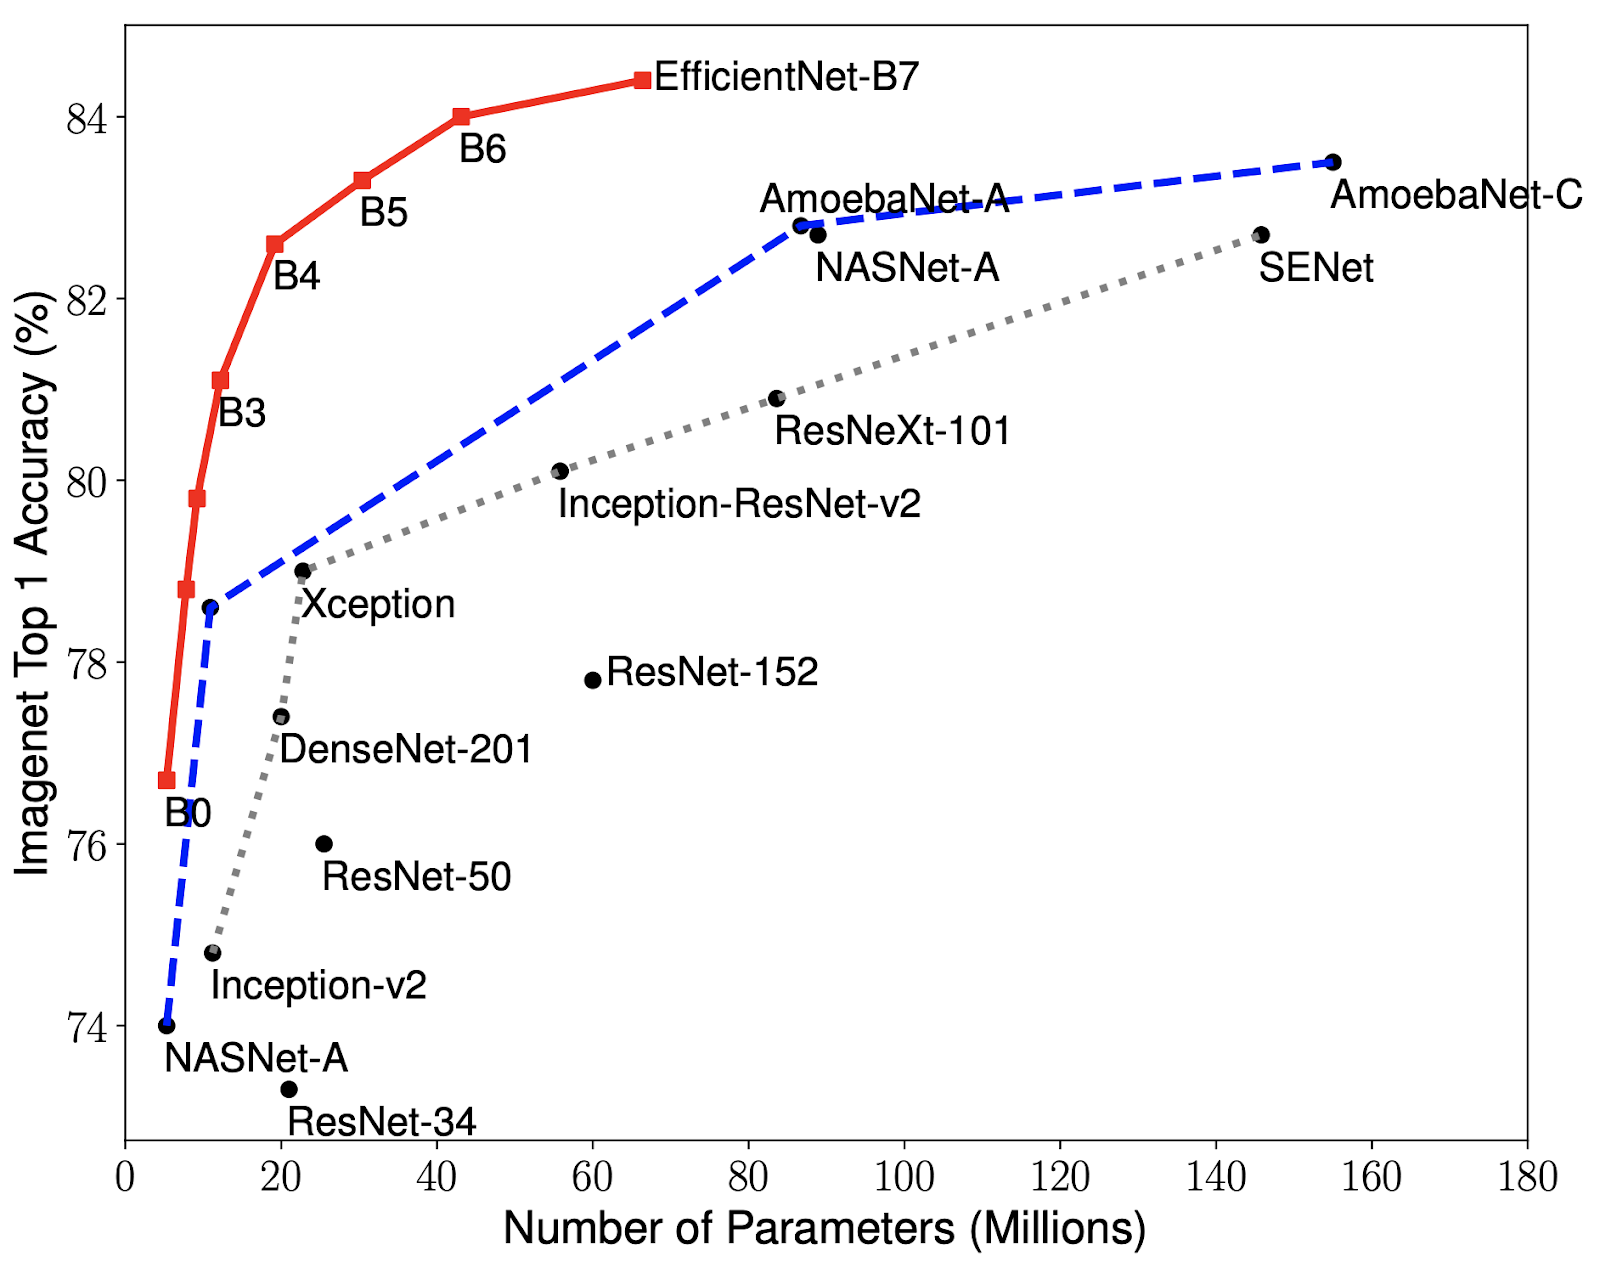
\includegraphics[width=0.9\columnwidth]{gambar/akurasiefn.png}
	
	% Ubah dengan keterangan gambar yang diinginkan
	\caption{Akurasi EfficientNet pada dataset \textit{ImageNet} \citep{cit:effnet}}
	\label{fig:akurasi-efn}
\end{figure}

EfficientNet juga diuji pada dataset lainnya dan mendapatkan akurasi \textit{state-of-the-art} pada 5 dari 8 dataset yang umum digunkan, diantaranya CIFAR-100(91.7\%) dan Flowers(98.9\%).
  \cleardoublepage

  % Bab 3 desain dan implementasi
  \chapter{DESAIN DAN IMPLEMENTASI}
\label{chap:desainimplementasi}

% Ubah bagian-bagian berikut dengan isi dari desain dan implementasi

Penelitian ini dilaksanakan sesuai \lipsum[1][1-5]

\section{Deskripsi Sistem}
\label{sec:deskripsisistem}

Sistem akan dibuat dengan \lipsum[1-2]

\section{Implementasi Alat
\label{sec:implementasi alat}}

Alat diimplementasikan dengan \lipsum[1]

% Contoh pembuatan potongan kode
\begin{lstlisting}[
  language=C++,
  caption={Program halo dunia.},
  label={lst:halodunia}
]
#include <iostream>

int main() {
    std::cout << "Halo Dunia!";
    return 0;
}
\end{lstlisting}

\lipsum[2-3]

% Contoh input potongan kode dari file
\lstinputlisting[
  language=Python,
  caption={Program perhitungan bilangan prima.},
  label={lst:bilanganprima}
]{program/bilangan-prima.py}

\lipsum[4]

  \cleardoublepage

  % Bab 4 pengujian dan analisis
  \chapter{PENGUJIAN DAN ANALISIS}
\label{chap:pengujiananalisis}

% Ubah bagian-bagian berikut dengan isi dari pengujian dan analisis

Pada penelitian ini dipaparkan \lipsum[1][1-5]

\section{Skenario Pengujian}
\label{sec:skenariopengujian}

Pengujian dilakukan dengan \lipsum[1-2]

\section{Evaluasi Pengujian}
\label{sec:analisispengujian}

Dari pengujian yang \lipsum[1]

% Contoh pembuatan tabel
\begin{longtable}{|c|c|c|}
  \caption{Hasil Pengukuran Energi dan Kecepatan}
  \label{tb:EnergiKecepatan}\\
  \hline
  \rowcolor[HTML]{C0C0C0}
  \textbf{Energi} & \textbf{Jarak Tempuh} & \textbf{Kecepatan} \\
  \hline
  10 J & 1000 M & 200 M/s \\
  20 J & 2000 M & 400 M/s \\
  30 J & 4000 M & 800 M/s \\
  40 J & 8000 M & 1600 M/s \\
  \hline
\end{longtable}

\lipsum[2-4]

  \cleardoublepage

  % Bab 5 penutup
  \chapter{PENUTUP}
\label{chap:penutup}

% Ubah bagian-bagian berikut dengan isi dari penutup

\section{Kesimpulan}
\label{sec:kesimpulan}

Berdasarkan hasil pengujian dan analisis yang telah dilakukan pada BAB 4, didapat kesimpulan sebagai berikut sebagai berikut:

\begin{enumerate}[nolistsep]

  \item Pada Pengujian berdasarkan sudut pengambilan video, Apabila sudut terlampau jauh dari sudut pengambilan video pada dataset, maka akurasi sistem menurun

  \item Pada Pengujian berdasarkan setup pengambilan video, Apabila setup yang digunakan menyebabkan perubahan bentuk pada citra, maka akurasi sistem akan menurun

  \item Dataset yang dimiliki masih dirasa kurang untuk mendapat model klasifikasi gerakan cuci tangan yang lebih general / dapat digunakan pada skenario yang lebih luas

\end{enumerate}

\section{Saran}
\label{chap:saran}

Untuk pengembangan lebih lanjut pada Sistem Klasifikasi Gerakan Mencuci Tangan ini, dapat dilakukan berberapa hal antara lain:

\begin{enumerate}[nolistsep]

  \item Untuk menggunakan sistem ini secara realtime, dapat dilakukan pemilihan model yang lebih cepat dan pemilihan metode input dan output yang lebih efisien.
  
  \item Untuk meningkatkan efisiensi training, dapat dilakukan optimasi kode program dan \textit{Hyperparameter} yang lebih mendalam

  \item Untuk meningkatkan efisiensi training, dapat pula sistem dapat dikembangkan sebuah metode untuk mengekstrak bagian tangan dan memisahkannya dari background ke dalam sistem klasifikasi ini

  \item Untuk meningkatkan kememampuan \textit{generalization} dari sistem klasifikasi ini, dapat dilakukan dengan penambahan jumlah Training Dataset dari sumber dan setup pengambilan yang lebih beragam, sehingga sistem lebih leluasa digunakan pada situasi dan setup yang berbeda

\end{enumerate}

  \cleardoublepage

  % Daftar pustaka
  \renewcommand\bibname{DAFTAR PUSTAKA}
  \addcontentsline{toc}{chapter}{\bibname}
  \bibliographystyle{unsrtnat}
  \bibliography{pustaka/pustaka.bib}
  \cleardoublepage

  % Biografi penulis
  \begin{center}
  \Large
  \textbf{BIOGRAFI PENULIS}
\end{center}

\addcontentsline{toc}{chapter}{BIOGRAFI PENULIS}

\vspace{2ex}

\begin{wrapfigure}{L}{0.3\textwidth}
  \centering
  \vspace{-3ex}
  % Ubah file gambar berikut dengan file foto dari mahasiswa
  
\includegraphics[width=0.3\textwidth]{gambar/elon.jpg}
  \vspace{-4ex}
\end{wrapfigure}

% Ubah kalimat berikut dengan biografi dari mahasiswa
Elon Reeve Musk, lahir pada \lipsum[1]

\lipsum[2]

  \cleardoublepage

\end{document}
